\documentclass[master,
               oneside,
               BCOR=10mm,
               ngerman,
               english,
               final,          %% Endversion; draft fuer schnelles Kompilieren
               ]{GAUBM}

\usepackage{float}
\usepackage{graphicx}
\usepackage{placeins}
\usepackage{wrapfig} 
\usepackage{setspace}
\usepackage{babel}
\usepackage{calc}
\usepackage[T1]{fontenc}
\usepackage[utf8]{inputenc}
\usepackage{caption}  % important
\usepackage[labelfont=bf]{caption}  % important
\usepackage{subcaption} % important
\usepackage{amsmath,amssymb, amsfonts}
\usepackage{mathrsfs}
\usepackage{longtable}
\usepackage{booktabs}
\usepackage{hhline}
\usepackage{array}
\usepackage{dcolumn}
\usepackage{bm}
\usepackage{siunitx}
\usepackage{xspace}
\usepackage{lmodern}
\usepackage[comma,numbers,sort&compress]{natbib}


\makeatletter
\newcommand{\subrefb}[1]{(\subref{#1})}
\makeatother
\bibliographystyle{bthesis}

\usepackage{longtable}
%\usepackage[it, bf]{caption}
\usepackage{amsfonts}
\usepackage{amsmath}
\usepackage{mathrsfs}
\usepackage{epsfig}
%\usepackage[clearempty]{titlesec}
\usepackage{booktabs}
\usepackage{hhline}
\usepackage{array}
\usepackage{floatflt}
\usepackage{graphicx}
\usepackage{dcolumn}
\usepackage{bm}
\usepackage{mathrsfs} 
\usepackage{amssymb}
\usepackage{siunitx}

\usepackage{amsfonts}
\usepackage{amsmath}
\usepackage{mathrsfs}
\usepackage{xspace}
%

\sisetup{
  inter-unit-product 	=	$\cdot$,
  fraction-function   	= 	\nicefrac,
  load-configurations 	= 	abbreviations,
  per-mode            	= 	fraction,
  separate-uncertainty	=	true,
  output-decimal-marker	=	{.}
  }
\DeclareSIUnit\barn{b}
\usepackage{float}


\setlength{\oddsidemargin}{0cm}
\setlength{\evensidemargin}{0cm}
\setlength{\topmargin}{-1cm}
\setlength{\textheight}{23cm}
\setlength{\textwidth}{16cm}
\setlength{\parindent}{0cm}

\pagestyle{headings}

\renewcommand{\sectfont}{\bfseries\rmfamily}
\renewcommand{\floatpagefraction}{0.7}
\renewcommand{\textfraction}{0.1}

% Experiments
\newcommand{\dzero}      {D\O\xspace}
\newcommand{\cdf}        {CDF\xspace}
\newcommand{\uubar}      {\mbox{$u\bar{u}$}\xspace}
\newcommand{\ddbar}      {\mbox{$d\bar{d}$}\xspace}
\newcommand{\ccbar}      {\mbox{$c\bar{c}$}\xspace}
\newcommand{\ssbar}      {\mbox{$s\bar{s}$}\xspace}
\newcommand{\ttbar}      {\mbox{$t\bar{t}$}\xspace}
\newcommand{\bbbar}      {\mbox{$b\bar{b}$}\xspace}
\newcommand{\wjets}      {\mbox{$W + 4\; jets$}\xspace}
\newcommand{\pttbar}     {\mbox{$p_{t\bar{t}}$}\xspace}
\newcommand{\pwjets}     {\mbox{$p_{W +4 \; jets}$}\xspace}
\newcommand{\ljets}      {\mbox{$\ell$+jets}\xspace}
\newcommand{\ejets}      {\mbox{$e$+jets}\xspace}
\newcommand{\mujets}     {\mbox{$\mu$+jets}\xspace}

% Laboratories
\newcommand{\fermilab}  {{F{\textsc{ermilab}}}\xspace}
\newcommand{\tevatron}  {{T{\textsc{evatron}}}\xspace}
\newcommand{\opal}      {{O{\textsc{pal}}}\xspace}
\newcommand{\cern}      {{C{\textsc{ern}}}\xspace}
\newcommand{\fnal}      {{F{\textsc{nal}}}\xspace}
\newcommand{\atlas}     {{A{\textsc{tlas}}}\xspace}
\newcommand{\lhc}       {{L{\textsc{hc}}}\xspace}
\newcommand{\lhcb}      {{L{\textsc{hc}}}{\scriptsize{b}}\xspace}
\newcommand{\lep}       {{L{\textsc{ep}}}\xspace}
\newcommand{\slc}       {{S{\textsc{lc}}}\xspace}
\newcommand{\pep}       {{P{\textsc{ep}}}\xspace}
\newcommand{\petra}     {{P{\textsc{etra}}}\xspace}
\newcommand{\hera}      {{H{\textsc{era}}}\xspace}
\newcommand{\lepaleph}  {{A{\textsc{leph}}}\xspace}
\newcommand{\delphi}    {{D{\textsc{elphi}}}\xspace}
\newcommand{\leplthree} {{L{\textsc{3}}}\xspace}
\newcommand{\lepopal}   {{O{\textsc{pal}}}\xspace}
\newcommand{\doris}     {{D{\textsc{oris}}}\xspace}
\newcommand{\isr}       {{I{\textsc{sr}}}\xspace}
\newcommand{\desy}      {{D{\textsc{esy}}}\xspace}
\newcommand{\kek}       {{K{\textsc{ek}}}\xspace}
\newcommand{\slac}      {{S{\textsc{lac}}}\xspace}
\newcommand{\tristan}   {{T{\textsc{ristan}}}\xspace}
\newcommand{\cms}       {{C{\textsc{ms}}}\xspace}
\newcommand{\alice}     {{A{\textsc{lice}}}\xspace}
\newcommand{\zeus}      {{Z{\textsc{eus}}}\xspace}
\newcommand{\hone}      {{H{\textsc{1}}}\xspace}
\newcommand{\minuit}    {{M{\textsc{inuit}}}\xspace}
\newcommand{\herwig}    {{H\textsc{erwig}}\xspace}
\newcommand{\acermc}    {{A\textsc{cerMC}}\xspace}
\newcommand{\evtgen}    {{E\textsc{vtgen}}\xspace}
\newcommand{\mcfm}      {{M\textsc{cfm}}\xspace}
\newcommand{\mcatnlo}   {{M\textsc{c@nlo}}\xspace}
\newcommand{\sherpa}    {{S\textsc{herpa}}\xspace}
\newcommand{\jimmy}     {{J\textsc{immy}}\xspace}
\newcommand{\cteq}      {{C\textsc{teq}}\xspace}
\newcommand{\pythia}    {{P\textsc{ythia}}\xspace}
\newcommand{\jetnet}    {{J\textsc{etnet}}\xspace}
\newcommand{\isajet}    {{I\textsc{sajet}}\xspace}
\newcommand{\jetset}    {{J\textsc{etset}}\xspace}
\newcommand{\vecbos}    {{V\textsc{ecbos}}\xspace}
\newcommand{\alpgen}    {{A\textsc{lpgen}}\xspace}
\newcommand{\vegas}     {{V\textsc{egas}}\xspace}
\newcommand{\gnu}       {{G\textsc{nu}}\xspace}
\newcommand{\onetop}    {{O\textsc{neTop}}\xspace}
\newcommand{\ztop}      {{Z\textsc{Top}}\xspace}
\newcommand{\toprex}    {{T\textsc{opRex}}\xspace}
\newcommand{\singletop} {{S\textsc{ingleTop}}\xspace}
\newcommand{\madgraph}  {{M\textsc{adgraph}}\xspace}
\newcommand{\madevent}  {{M\textsc{adevent}}\xspace}
\newcommand{\comphep}   {{C\textsc{omphep}}\xspace}
\newcommand{\qq}        {{Q\textsc{q}}\xspace}
\newcommand{\tauola}    {{T\textsc{auola}}\xspace}
\newcommand{\geant}     {{G\textsc{eant}}\xspace}
\newcommand{\GEANT}     {{G\textsc{eant}}\xspace}
\newcommand{\amegic}    {{A\textsc{megic++}}\xspace}

\newcommand{\met}       {\mbox{$\not\!\!E_{\mathrm{T}}$}\xspace}
\newcommand{\metcal}    {\mbox{$\not\!\!E_{Tcal}$}\xspace}
\newcommand{\MET}       {$\not\!\!E_{\mathrm{T}}$}
\newcommand{\lowmet}    {low-\mbox{$\not\!\!E_{\mathrm{T}}$}-QCD\xspace}
\newcommand{\lumi}      {$\mathcal{L}$\xspace}
\newcommand{\intlumi}   {$\int\mathcal{L}\,\mathrm{d}t$\xspace}

\newcommand{\runi}      {Run~I\xspace}  %% For Tevatron! (Roman numerals)
\newcommand{\runii}     {Run~II\xspace}
\newcommand{\LHCruni}   {Run~1\xspace}  %% For LHC! (Arabic numerals)
\newcommand{\LHCrunii}  {Run~2\xspace}
\newcommand{\LHCruniii}  {Run~3\xspace}

\newcommand{\tabheadfont}[1]{\textbf{#1}}

\usepackage{textcomp,gensymb}
\usepackage[colorlinks=false,
            pdfstartview=FitH,
            breaklinks=true,
            bookmarksopen=true,
            bookmarksnumbered=true
            ]{hyperref}
\usepackage{cleveref}


\begin{document}

\ThesisAuthor{Siemen Henning}{Aulich}
\PlaceOfBirth{Emden}
\ThesisTitle{Improving Event Reconstruction for Dileptonic Decays of Top Quarks Pairs Using Machine Learning}{}%{Verbesserung der Event Rekonstruktion für dilpetonische Zerfälle von Top Quark Paaren mit Machine Learning}
\FirstReferee{Prof.~Dr.~Stan Lai}
\Institute{DESY Hamburg}
\SecondReferee{Dr.~Katharina Behr}

\CourseName{M.Phy.1610: Development and Realization of Scientific
Projects in Theoretical Physics}


\ThesisBegin{7}{4}{2025}
\ThesisEnd{4}{12}{2026}

\frontmatter
\maketitle
\cleardoublepage
\begin{abstract}
  \noindent Many of the recent highlights in particle physics research are related to top quark physics'. These include both the stringent tests of spin correlations and quantum effects in pairs of top quarks ($t\bar{t}$), and the observation of a possible quasi-bound state resonance in the $t\bar{t}$
  invariant mass spectrum. The latter presents a very exciting opportunity to extend our current understanding of non-relativistic Quantum Chromodynamics. Both effects are predominantly studied in the dilepton decay channel of the top quark in a mass range close to the $t\bar{t}$ production threshold.

  The dilepton final state contains two neutrinos, besides two charged leptons and two b-quark jets. Probing this system requires a precise reconstruction of the top quarks, which is complicated by the presence of the two neutrinos.  While analytical regression strategies primarily focus on inferring the neutrino momenta, the problem of correctly assigning b-jets to their parent top quarks remains largely understudied. However, many of the sensitive variables used in $t\bar{t}$  precision measurements depend critically on the correct assignment of the jets.

  Inspired by the success of machine learning architectures in tackling the assignment challenge for hadronic decay channels, this work investigates using a transformer model for the dilepton channel. An architecture specifically tailored to this channels topology is shown to outperform all existing methods in assigning reconstructed particles to their parent partons, improving the resolution of relevant physics observables. Furthermore, it is investigated how these efforts can be combined with neutrino regression methods to offer a full reconstruction pipeline. Applying these methods to existing and upcoming analyses promises further enhancements in the sensitivity and precision of searches and measurements alike.
  \bigskip\par
  \textbf{Keywords:} Top Quark, Machine Learning, Event Reconstruction, Dilepton Channel, Transformer Networks
\end{abstract}

\cleardoublepage
\tableofcontents
\mainmatter

\chapter{Introduction}
\label{chap:introduction}
The top quark, being the heaviest known elementary particle, plays a crucial role in the Standard Model of particle physics. Its unique properties and interactions make it an excellent probe for testing the limits of our current understanding of fundamental forces and searching for potential new physics beyond the Standard Model. It is one of the most studied processes at the Large Hadron Collider (\lhc) at \cern.
Top quarks are predominantly produced in pairs (\ttbar) via the strong interaction in proton-proton collisions at the \lhc. Each top quark decays almost exclusively into a W boson and a b-quark. The W boson can further decay either leptonically (into a charged lepton and a neutrino) or hadronically (into a pair of quarks). The dileptonic decay channel, where both W bosons decay leptonically, results in a final state with two charged leptons, two b-jets, and two neutrinos. This channel, while having a lower branching ratio compared to other decay modes, offers a cleaner experimental signature due to the presence of high-\pt leptons and reduced hadronic activity. However, the presence of two neutrinos in the final state poses significant challenges for event reconstruction, as they evade detection, leading to missing transverse energy (\met) in the event.

Due to its clean signature and sensitivity to various top quark properties, the dileptonic \ttbar channel is widely used for precision measurements of the top properties or spin correlations. Two recent highlights in top quark physics are the stringent tests of spin correlations and quantum effects in pairs of top quarks, and the observation of a possible quasi-bound state resonance in the $t\bar{t}$ invariant mass spectrum. Both effects are predominantly studied in the dilepton decay channel of the top quark in a mass range close to the $t\bar{t}$ production threshold. The latter presents a very exciting opportunity to extend our current understanding of non-relativistic Quantum Chromodynamics.

Both analyses rely on measurements of angular distributions and correlations between the decay products of the top quarks. Probing this system requires a precise reconstruction of the top quarks, which is complicated by the presence of the two neutrinos. While analytical neutrino regression strategies have been studied extensively, the problem of correctly assigning b-jets to their parent top quarks remains largely unstudied. In the all-hadronic and lepton+jets channels, various methods for jet assignment have been developed and employed successfully. However, in the dileptonic channel, the jet assignment problem was often simplified or overlooked due to a focus on neutrino reconstruction. However, many of the sensitive variables used in $t\bar{t}$ precision measurements depend critically on the correct assignment of the jets. Misassignments can lead to significant biases and degrade the resolution of reconstructed observables, ultimately limiting the precision of measurements.

Inspired by the success of machine learning architectures in tackling the assignment challenge for hadronic decay channels, this work investigates using a transformer model for the dilepton channel. It introduces the necessary theoretical background in \Cref{chap:background} before detailing the use of machine learning in particle physics in \Cref{chap:machine-learning}. The reconstruction methods are outlined in \Cref{chap:reconstruction-methods}, followed by the development of the machine learning-based jet assignment in \Cref{chap:ml-jet-selection}. For this, different transformer architectures are explored and optimized. The performance of the developed methods is evaluated in \Cref{chap:performance-evaluation}, where thee impact on relevant physics observables is assessed. Finally, \Cref{chap:conclusion} summarizes the findings and discusses potential future directions for further improving dileptonic \ttbar event reconstruction.
\chapter{Theoretical Background}
\label{chap:background}
\section{The Standard Model of Particle Physics}
\label{sec:standard_model}
\begin{figure}[h]
    \centering
    \includegraphics[width=0.8\textwidth]{figures/standard_model.pdf}
    \caption{The particles of the Standard Model. Particle porperties taken from Ref. \cite{PDG2024}.}
    \label{fig:standard_model_particles}
\end{figure}
The Standard Model of Particle Physics (SM) provides the theoretical foundation describing three of the four elementary forces as well the particles making up the known matter.\\
The Figure \ref{fig:standard_model_particles} shows a tabular overview of the known particle of the Standard Model.
The SM classifies the elementary particles into fermions and bosons.
Fermions are the building blocks of matter and have half-integer spin values. They are further divided into quarks and leptons.
Quarks experience all four fundamental forces, while leptons do not participate in the strong interaction.
Bosons are the force carriers of the fundamental interactions and have integer spin values.
The photon, W and Z bosons, and gluons mediate the electromagnetic, weak, and strong forces, respectively.
The Higgs boson is responsible for giving mass to other particles through the Higgs mechanism.\\
Based on the coupling of the weak interaction, two particles are grouped into one iso-spin doublet.
The iso-spin is the quantum number related to the weak interaction. Two quarks form one doublet and one lepton and its corresponding neutrino form another doublet.
Based on the different masses, two iso-spin doublets are grouped into what is called a generation.
There are three generations of fermions, with each generation containing heavier particles than the previous one.

\section{Top Quark Physics}
\label{sec:top_quark_physics}
The positive iso-spin partner of the third generation quark doublet is the top quark ($t$). With a mass of about $173\,\mathrm{GeV}/c^2$ \cite{PDG2024}, it is the heaviest known elementary particle.
Due to its high mass, the top quark has a very short lifetime of approximately $5\times10^{-25}\,\mathrm{s}$ \cite{PDG2024}, which is shorter than the timescale for hadronization.

\chapter{Machine Learning in High Energy Physics}
Since this work focuses on improving the event reconstruction of dileptonic \ttbar decays using machine learning techniques, this chapter provides an overview of the fundamental concepts and methodologies employed in machine learning. 

\section{Supervised Learning}
Machine learning can be broadly categorized into supervised and unsupervised learning. In supervised learning, the model is trained on a labeled dataset, where each input data point is associated with a corresponding target output. The goal of the model is to learn a mapping from inputs to outputs, enabling it to make accurate predictions on unseen data.
\subsection{Monte Carlo Training Data}
In high energy physics, supervised learning is commonly performed by training mdoels on simulated datasets. The way the Monte Carlo Event modelling is performed in particle physics, makes it naturally suited for supervised learning tasks.\\
Events are usually simulated using a cascade of different programs, each simulating a different state of the event. First the hard scattering process is simulated using matrix element generators like \textsc{MadGraph} \cite{madevent_1} or \textsc{Powheg} \cite{powheg}. These programs calculate the probabilities of different particle interactions based on the underlying physics theories, such as the Standard Model. Using these probabilities, they generate events that represent the initial state of the particles after the collision. The possible kinematic phase space is sampled according to these probabilities, resulting in a set of particles with specific momenta and energies. This type of event variables is often referred to as \textit{parton-level}.\\
Next, the parton showering and hadronization processes are simulated using programs like \textsc{Pythia} \cite{pythia}. Parton showering models the emission of additional particles from the initial partons, while hadronization simulates the formation of hadrons from quarks and gluons. These processes are crucial for accurately modelling the final state particles observed in detectors.\\
Finally, detector simulation programs like \textsc{Geant4} \cite{geant4} are used to simulate the interaction of particles with the detector material, producing realistic detector responses. This includes simulating the energy deposits in calorimeters, hits in tracking detectors, and other relevant signals.\\
While the actual detector response is simulated using complex detector simulation software, for many machine learning applications, a simplified representation of the detector response is sufficient. This can involve smearing the particle momenta and energies according to the detector resolution, applying efficiency corrections, and simulating the effects of pile-up.\\
This is because, for the reconstruction of the physics objects, such as jets, leptons, and missing transverse energy, highly sophisticated algorithms are used that already take into account the detector effects (Note, that these algortihms may also be machine learning based,). Therefore, the input features for machine learning models can often be derived directly from these reconstructed objects, rather than relying on the raw detector signals. The reconstructed object event variables are called \textit{reco-level}.
\subsection{Training}
During the training phase, the model is presented with a set of input features derived from the reco-level event variables, along with their corresponding target outputs, which are typically derived from the parton-level event variables. The model learns to map the input features to the target outputs by minimizing a loss function that quantifies the difference between the predicted and true values. Common loss functions include mean squared error for regression tasks and cross-entropy \cite{cross-entropy} loss for classification tasks.\\
%\chapter{Experimental Setup}
\label{ch:exper_setup}
\section{The LHC}
The Large Hadron Collider (\lhc) at \cern is a synchrotron designed to accelerate protons and lead nuclei. This work focuses on the proton-proton collisions during \LHCrunii. During \LHCrunii from 2015 to 2018, the \lhc operated at a centre of mass energy of $\sqrt{s}=13\,\unit{\tera\electronvolt}$ with an integrated luminosity of $\mathcal{L}_{int}\approx 140\,\unit{\femto\barn^{-1}}$ \cite{ATLAS:2019pzw}.

After completion of \LHCruniii in June 2026 and an operational pause, the \lhc will operate with increased luminosity as the High-Luminosity Large Hadron Collider (HL-\lhc). During this phase, it is planned to accumulate data with an integrated luminosity of $\mathcal{L}=3\,\unit{\atto\barn^{-1}}$ \cite{Aberle:2749422}.
 \section{The Detector}
The \atlas detector is a general-purpose particle detector at the \lhc at \cern. It can roughly be separated into three elements: the inner detector, the calorimeter and the muon spectrometer \cite{atlas_tdr}.
\subsection{The Coordinate System}
The interaction point marks the origin of the \atlas coordinate system. The $z$-axis is orientated along the beamline, the $x$-axis points towards the centre of the \lhc and the $y$-axis points upwards.

Using this convention, several kinematic variables are defined. One of which is the transverse momentum defined as
\begin{align}
    p_T=\sqrt{p_x^2+p_y^2}
\end{align}
Because of the cylindrical shape of the \atlas detector and the cylindrical symmetry of the interactions, the azimuthal angle is used as another variable. The polar angle relative to the $z$-axis can be used to define the pseudorapidity which can also be expressed in terms of the momentum
\begin{align}
    \eta=-\ln\left(\tan\left(\frac{\theta}{2}\right)\right)=\ln\left(\frac{|\vec p|+p_z}{|\vec p|-p_z}\right)\,.
\end{align}
In the ultra-relativistic limit $m\ll |\vec p|$ the pseudorapidity is equal to the rapidity defined as
\begin{align}
    y=\frac{1}{2}\ln\left(\frac{E+p_z}{E-p_z}\right)\,.
\end{align}
These variables are convenient for the usage in the \atlas experiment because $p_T,\phi$, and differences of $\eta$ are invariant under Lorentz-boost along the $z$-axis.
\subsection{The Inner Detector}
\begin{figure}[ht]
    \centering
    \includegraphics[width=0.8\textwidth]{figures/atlas-detector/IDbriefing_figure1.png}
    \caption{Schematic cross-section of the inner detector of the \atlas detector (\copyright\ \cern).}
    \label{fig:inner_det}
\end{figure} \noindent
The inner detector (ID) is the innermost part of the \atlas detector. It is used for tracking charged particles, particle identification, and primary and secondary vertex determination \cite{atlas_tdr}. The ID consists of three different sub-detectors. Their rough structure is depicted in \Cref{fig:inner_det}. The ID is encapsulated with a solenoid magnet providing a $2\,\unit{\tesla}$ axial magnetic field on the inside of the ID. The magnetic field is crucial to measure the momentum of a charged particle. The transverse momentum is measured as the curvature of the particle's track due to the Lorentz force.

The detector part closest to the beam pipe is the pixel detector. It consists of 1744 modules arranged in three barrel layers. Each module hosts 47232 silicon pixels with a size of $50\times 400\,\unit{\micro \metre^2}$. The pixels are semiconductor trackers used to detect the traversing of charged particles.

The following part of the detector is the semiconductor tracker (SCT). It consists of 4088 modules arranged in four layers to guarantee four position measurements of charged particles. Each module consists of four silicon sensors. The sensors offer a $17\,\unit{\micro \metre}$ resolution in-plane lateral and $580\,\unit{\micro \metre}$ in-plane longitudinal.

The outermost part of the inner detector is the transition radiation tracker (TRT). It consists of polyimide drift (straw) tubes with a $4\,\unit{\milli\metre}$ diameter that are arranged in a $528\,\unit{\milli\metre}$ thick cylindrical layer around the beam pipe. The straw tubes are interleaved with fibres for the readout. The transition radiation tracker utilizes the transition light emitted by charged particles traversing the interface between two media with different indices of refraction. The TRT offers a measurement of charged particles and electron identification.
\subsection{Calorimeter}
\begin{figure}[ht]
    \centering
    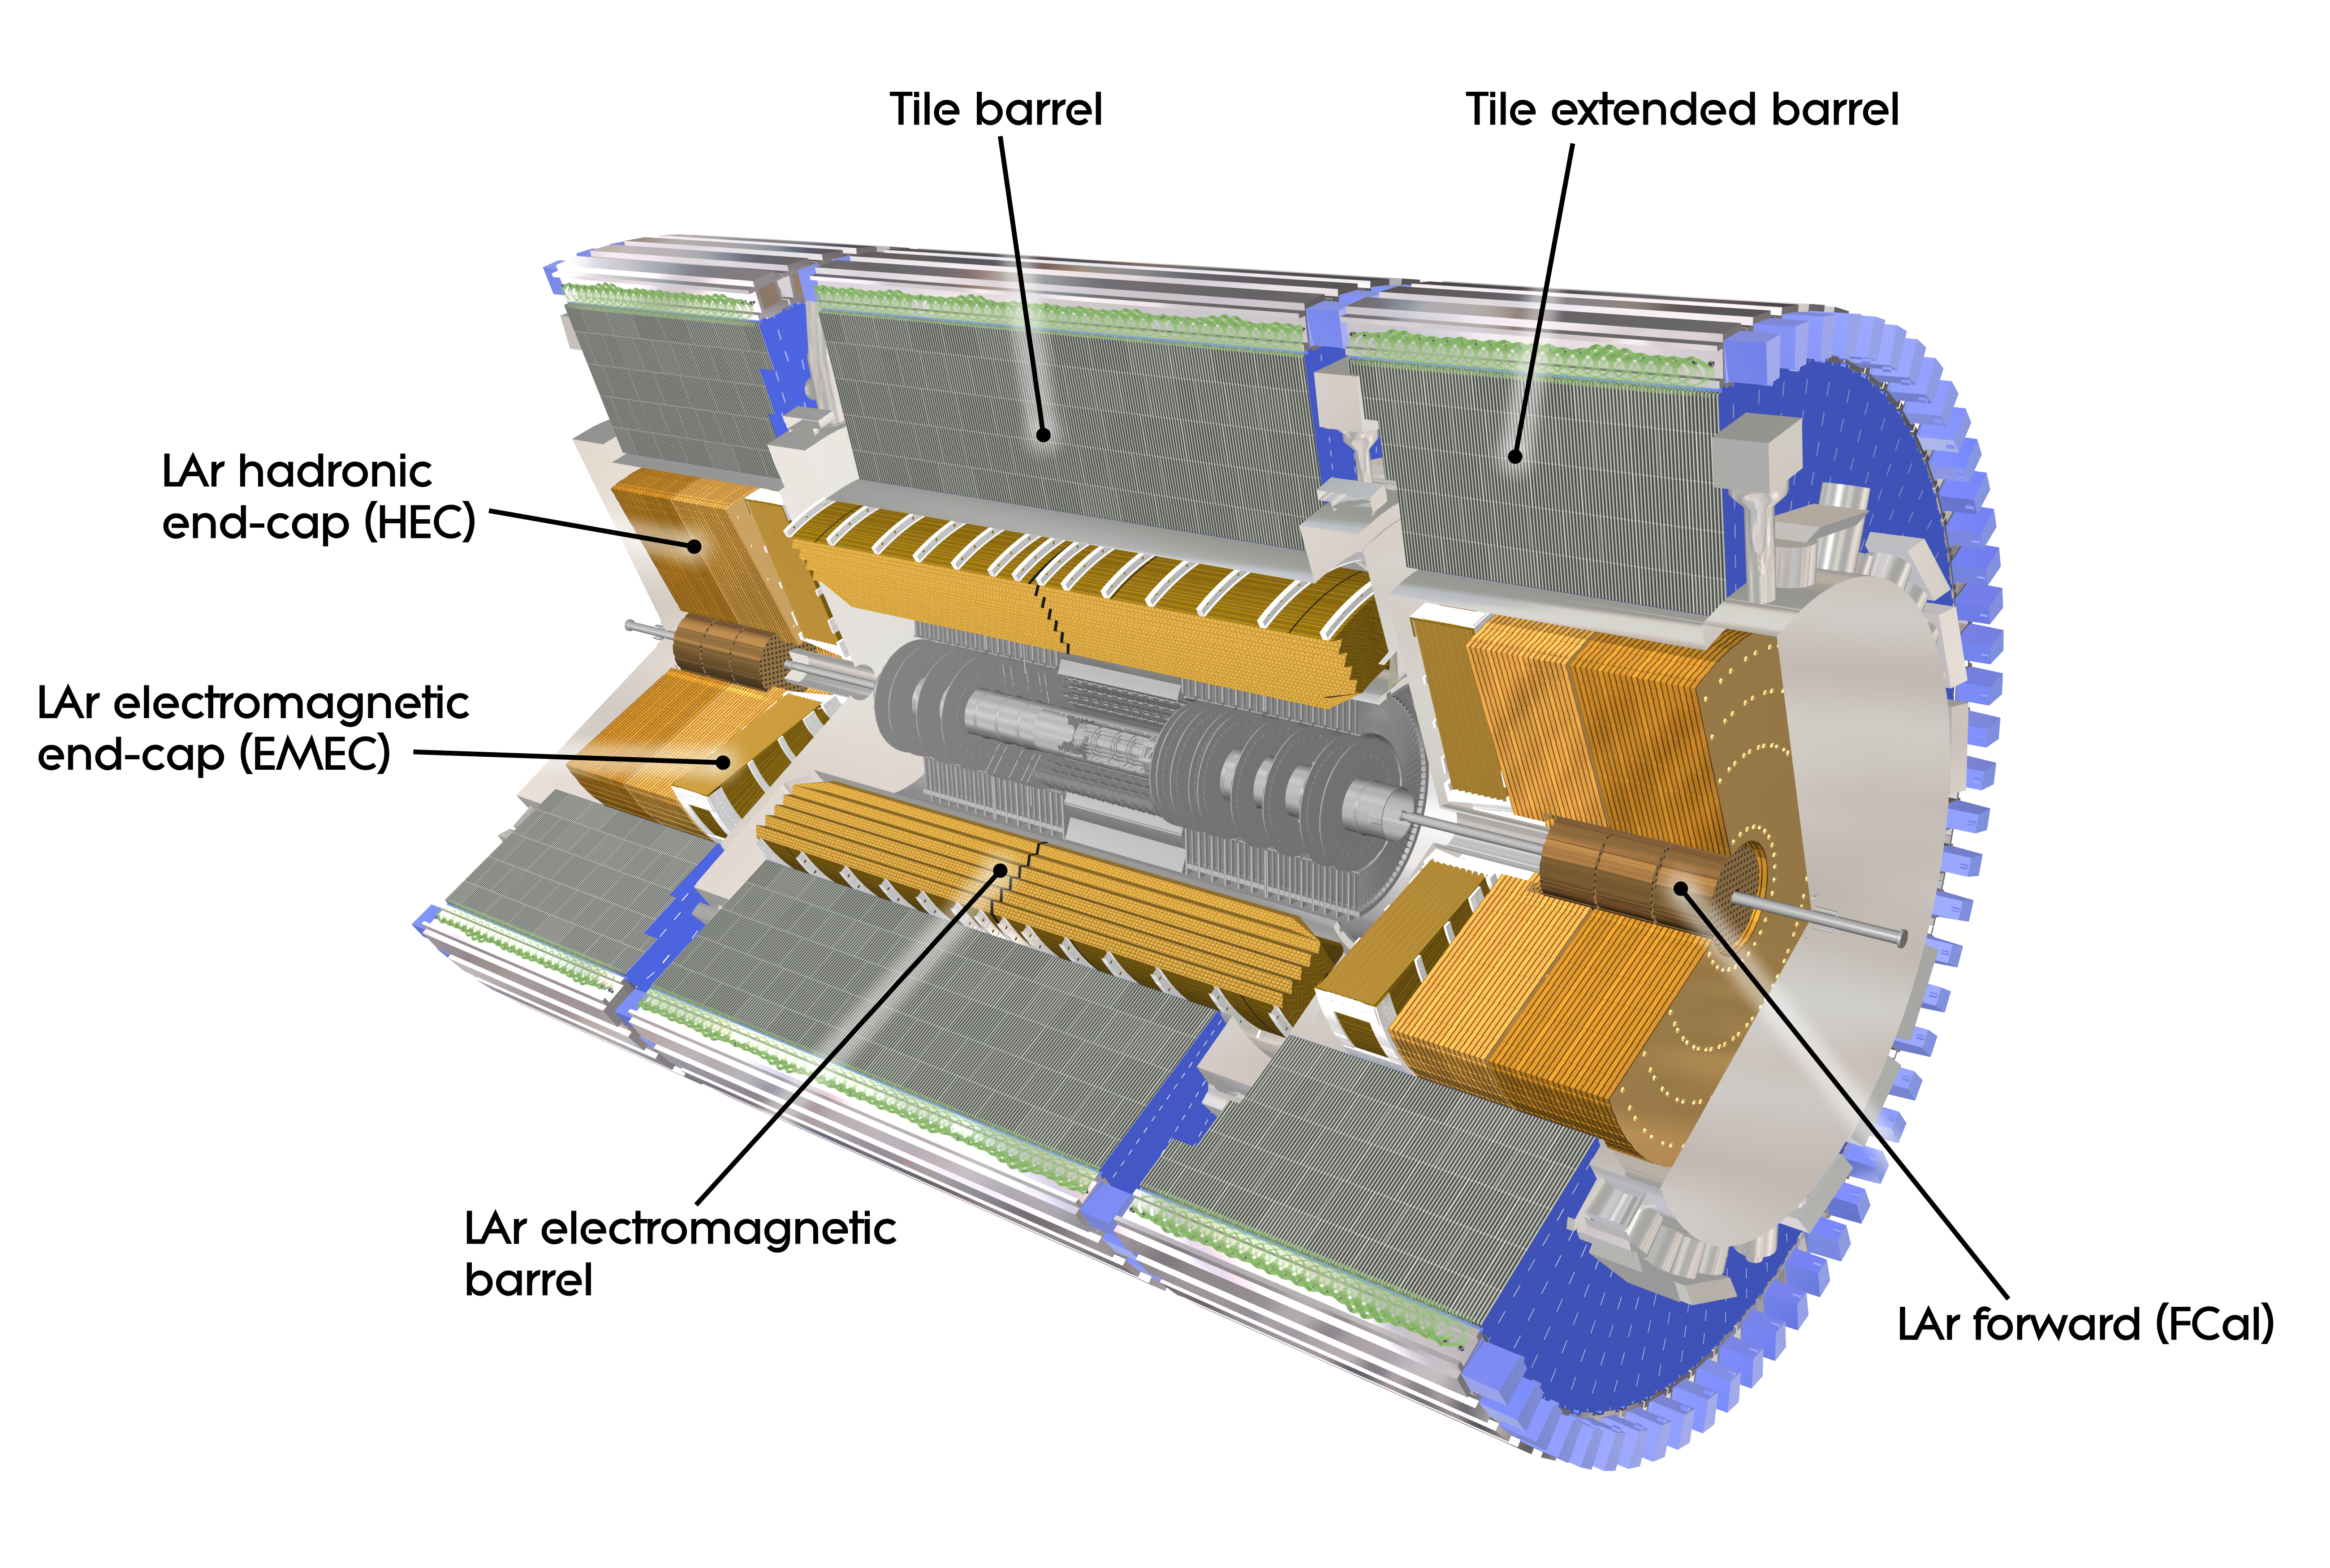
\includegraphics[width=0.7\textwidth]{figures/atlas-detector/0803015_01.jpg}
    \caption{Computer generated image of the \atlas calorimeter (\copyright\ \cern).}
    \label{fig:colorimeter}
\end{figure}\noindent
The calorimeters are the detector layers following the inner detectors. Its structure is divided into the Electromagnetic calorimeter (ECal) and the hadronic calorimeter (HCal).
\subsubsection{Electromagnetic Calorimeter}
The ECal is used for the energy and position measurement of electric charged particles and photons. It utilizes bremsstrahlung and pair production to create a cascade of charged particles which are measured. It offers full azimuthal coverage and is equipped with end caps in the longitudinal direction of the beam pipe. The \atlas ECal is a sampling calorimeter operating with lead as the passive and liquid Argon as the active medium. The innermost part of the ECal is a presampler which detects if the particle started showering before reaching the ECal.
\subsubsection{Hadronic Calorimeter}
The HCal measures the energy and position of baryons and mesons through strong interactions with the nuclei. In the range of $|\eta|<1.7$ it is a sampling calorimeter with steel as the passive and scintillators as the active medium. For the end cap, liquid Argon is deployed as the active medium. The HCal works with the same principle as the ECal but offers less precise measurements.

In the range of $3.1<|\eta|<4.9$ ECal and HCal are substituted with the forward calorimeters (FCal) which are made up of three modules to fulfil the function of both calorimeters.

In combination with the FCal a total range of $|\eta|<4.9$ is covered by the calorimeters.

A computer-generated image of the structure of the different calorimeters used in the \atlas detector is shown in \Cref{fig:colorimeter}.
\subsection{Muon Spectrometer}
The muon spectrometer is the outermost part of the \atlas detector. Its purpose is to detect charged particles exiting the calorimeters and measure their momentum in the range of $|\eta|<2.7$. A detector dedicated to the measurement of muons is necessary because their mass makes them minimal ionizing particles in the energy range of the \lhc collisions. The amount of energy loss due to bremsstrahlung is not sufficient to develop showers necessary to measure their energy. The muons' transverse momenta can be measured in the ID. Like the inner detector, the muon spectrometer utilizes a magnetic field to conduct a measurement of the particle's momentum.  In the muon spectrometer, however, a solenoid magnet is used to allow for the measurement of the muon's momentum along a different direction. Combining the measurements, one obtains full knowledge of the muons four-momentum. Further, does the high rate of stopped electrons and hadrons in the calorimeters enable a high specificity in the muon detection.


\subsection{Trigger System}
With a bunch spacing of $25\,\unit{\nano\second}$ \cite{ATLAS:2019pzw} collisions happen at a rate of $40\,\unit{\mega\hertz}$. Each collision involves up to hundreds of particles. To reduce the data to a feasible amount, triggers are employed to filter less interesting events. Different layers of triggers operate either at the hardware or software level. The L1 trigger is a hardware level trigger and acts as the first filter for the events. It makes decisions in less than $2.5\,\unit{\micro\second}$. The subsequent L2 trigger is a software level trigger and makes decisions in less than $200\,\unit{\micro \second}$. Combined, the trigger system reduces the event rate from $40\,\unit{\mega\hertz}$ to $1000\,\unit{\hertz}$ which are then stored at the \cern data centre.

\chapter{Analysis and Reconstruction}
\label{chap:reconstruction-methods}
\section{Data and Simulation}
\label{sec:data-and-simulation}

This section describes the data and simulation samples used in this analysis. At the current stage of this thesis, only simulation samples have been studied; the data samples will be described in the final version. The simulated samples are produced using Monte Carlo (MC) event generators, which model the physics processes occurring in proton-proton collisions at the LHC.

While a complete analysis requires detailed investigation of background processes contributing to the signal regions, this thesis focuses on developing and evaluating reconstruction methods. Therefore, only the signal process of \ttbar production with dileptonic decays is described here. The background processes and their simulation will be discussed in the final thesis.

\subsection{Simulation of Dileptonic Top Quark Pair Events}

The signal process of \ttbar production with dileptonic decays is simulated using \powheg~\cite{powheg} at next-to-leading order (NLO) in perturbative quantum chromodynamics (QCD). The \powheg generator is interfaced with \pythia~\cite{pythia} for parton showering, hadronization, and underlying event modelling.

To link the reco-level particles to the parton-level objects, a parton matching is performed. The parton-level objects are defined as the top quarks and their decay products after final state radiation before hadronization. The matching is done by iteratively associating reconstructed jets to partons based on angular distance criteria. The decay products of the top quarks are matched within a cone of $\Delta R \leq 0.3$ and $\Delta R\leq 0.1$ for jets and leptons ($e$,$\mu$) respectively. If multiple reconstructed objects are found within this cone, the one with the smallest $\Delta R$ is chosen.


\subsection{Object Definition}

The reconstruction of physics objects—electrons, muons, jets, and missing transverse energy (\met)—is performed using the standard \atlas reconstruction algorithms~\cite{atlas_tdr}.

\paragraph{Electrons} are required to have transverse momentum \pt $> 5~\unit{\giga\electronvolt}$ and pseudorapidity $|\eta| < 2.47$, excluding the transition region between the barrel and endcap calorimeters ($1.37 < |\eta| < 1.52$). Electrons must satisfy the Tight identification criteria and be isolated from other activity in the detector.

\paragraph{Muons} are reconstructed using information from both the inner detector and the muon spectrometer. They are required to have \pt $> 5~\unit{\giga\electronvolt}$ and $|\eta| < 2.5$. Muons must satisfy the Tight identification criteria and be isolated.

\paragraph{Jets} are reconstructed using the anti-$k_t$ algorithm \cite{anti_k_t_jet_2} with a radius parameter of $R = 0.4$. They are required to have \pt $> 25~\unit{\giga\electronvolt}$ and $|\eta| < 2.5$. B-tagging is performed using the GN2 algorithm~\cite{gn2_btagger} to identify jets originating from b-quarks.

\paragraph{Missing Transverse Energy} (\met) is calculated from the negative vector sum of the transverse momenta of all reconstructed objects.

\subsection{Event Selection}
Events are selected to contain exactly two oppositely charged leptons (electrons or muons). One of the leptons must have \pt $> 25~\unit{\giga\electronvolt}$, while the other must have \pt $> 5~\unit{\giga\electronvolt}$. At least two jets are required, with at least one being b-tagged at the $77\%$ working point (WP). Additional selection criteria are applied to suppress background contributions, which will be detailed in the final thesis.

For the training and evaluation of the reconstruction methods, only events that pass the selection criteria and have a successful parton matching are considered.

\section{Event Reconstruction}
\label{sec:reconstruction-methods}
Reconstructing the kinematics of dileptonic \ttbar events requires an assignment of reconstructed objects to the parton-level decay products. This section describes the different reconstruction methods developed and evaluated in this thesis.

While the leptons are directly identified from the reconstructed objects, the assignment of jets to the b-quarks from the top quark decays is ambiguous due to the presence of multiple jets in the event. Additionally, the two neutrinos from the W boson decays are not directly detected, leading to missing information in the event reconstruction.
Based on this, the reconstruction breaks down into two main tasks:
\paragraph{Neutrino Regression} Estimating the momenta of the two neutrinos using the measured \met and other event kinematics.
\paragraph{Jet Assignment} Assigning the reconstructed jets to the b-quarks from the top quark decays.
\subsection{Neutrino Regression Methods}
\label{sec:neutrino_regression}
Due to the current stage of the thesis, only one baseline method for neutrino regression has been used. The method of choice for the final thesis will be determined after evaluating multiple approaches.

The baseline method used here is called $\nu^2$-Flows \cite{nu_square_flows} and uses normalizing flows to model the conditional probability distribution of the neutrino momenta given the observed event kinematics. The model is trained on simulated dileptonic \ttbar events, where the true neutrino momenta are known from the parton-level information. The trained model can then be used to sample possible neutrino momenta for new events, allowing for a probabilistic reconstruction of the event kinematics. For each event, multiple samples of neutrino momenta are drawn from the model, and the one with the highest probability density is selected as the reconstructed neutrino momenta.
A detailed outline of the $\nu^2$-Flows method and its implementation can be found in Ref.~\cite{nu_square_flows}. For this thesis, this method serves to establish a baseline for neutrino regression to evaluate the impact of improved jet assignment methods. Note, however, that this method has not been used in \atlas analyses yet. However, due to matters of software compatibility, it was the only viable option at this stage of the thesis.
Since, $\nu^2$-Flows processes the full event information to make a prediciton for the neutrino momenta, it is agnostic to the jet assignment. This is drastically different from the conventional methods, which were used in previous \atlas analyses \cite{entanglement_top_quarks}. Which are interdependent with the jet assignment. These are mostly based on exploiting the kinematic constraints of the event, such as the invariant masses of the W bosons and top quarks outlined in \Cref{sec:kinematic_constraints}.
\subsection{Jet Assignment Methods}
\label{sec:jet_assignment}
This thesis explores several methods for jet assignment, ranging from traditional algorithms to machine learning approaches. From recent publications e.g. \cite{entanglement_top_quarks}, two conventional methods have been implemented as baselines:

\paragraph{Jet-Selection}
Both methods start by selecting the two $b$-jet candidates in the event based on the $b$-tagging at the $77\%$ WP. If more than two $b$-tagged jets are present, the two with the highest \pt are chosen. If only one $b$-tagged jet is found, the non-tagged jet with the highest $b$-tagging score is selected as the second candidate.
\begin{figure}[H]
    \centering
    \begin{minipage}[t]{0.48\textwidth}
        \textbf{$\chi^2$-Method}\\[0.5em]
        For both possible assignments of the two b-jet candidates to the parton-level $b$-quarks, the invariant masses of the reconstructed top quarks are computed
        \begin{equation}
            \label{eq:chi_square}
            \chi^2 = (m_{b_1,{\nu},\ell^+} - m_{t})^2+(m_{b_2,\bar{\nu},\ell^-} - m_{t})^2
        \end{equation}
        where $m_t = 172.5~\unit{\giga\electronvolt}$ is the top quark mass. The assignment with the smaller $\chi^2$ value is chosen.
    \end{minipage}
    \hfill
    \begin{minipage}[t]{0.48\textwidth}
        \textbf{$\Delta R$-Method}\\[0.5em]
        This method assigns the $b$-jet candidates based on their angular distance to the leptons. 
        \begin{equation}
            \Delta R = \sqrt{(\Delta\phi)^2 + (\Delta\eta)^2}
        \end{equation}
        The jet lepton pair with the smaller $\Delta R$ value is assigned to each other. The remaining jet is assigned to the other lepton.
    \end{minipage}
\end{figure}
Note, that the $\chi^2$-Method relies on the reconstructed neutrino momenta to compute the invariant masses of the top quarks. Therefore, it is inherently linked to the neutrino regression method used. In contrast, the $\Delta R$-Method is independent of the neutrino momenta.
Further, it should be noted, that due to its reliance on the neutrino reconstruction and the use of $\nu^2$-Flows here, the $\chi^2$-method should also be considered a maching learning based approach.

The $\Delta R$-Method was used in previous \atlas analyses \cite{entanglement_top_quarks} for events, that failed the kinematic reconstruction required for the $\chi^2$-Method. However, in this thesis, both methods are evaluated on the full dataset for comparison.
\chapter{Machine Learning Based Jet Assignment}
\label{chap:ml-jet-selection}

In addition to the conventional jet assignment methods described in \Cref{sec:jet_assignment}, this thesis investigates machine learning-based approaches to improve the accuracy of jet assignment in dileptonic \ttbar events. Machine learning techniques have shown promise in various aspects of high-energy physics, such as flavour tagging \cite{flavour_tagging_review}.

For the high permutation complexity of jet assignments in the all-jets channel, SPANet \cite{spanet} has demonstrated significant improvements over traditional methods. These architectures leverage attention mechanisms to improve the accuracy.
Based on these successes, this thesis explores the adaptation of similar architectures for the dileptonic \ttbar channel, which presents unique challenges due to the presence of two neutrinos and fewer jets.

Albeit a variety of architectures were tested during the development (including RNNs), two manifested as the best performing ones.

\section{Neural Network Architectures}
\subsection{FeatureConcatTransformer}
\begin{figure}[H]
    \centering
    \includegraphics[width=1.\textwidth]{figures/machine-learning/feature_concat_transformer.pdf}
    \caption{Schematic of the \textbf{FeatureConcatTransformer} architecture.}
    \label{fig:feature_concat_transformer}
\end{figure}
The \textbf{FeatureConcatTransformer} architecture, illustrated in \Cref{fig:feature_concat_transformer} consists of the following components:
\begin{itemize}
    \item \textbf{Input Features:} The model takes as input a set of features for each reconstructed object (jets and leptons), including kinematic variables ($E$, \pt, $\eta$, $\phi$), $b$-tag score working point, and event-level features such as missing transverse energy (\MET). The features of both leptons and the missing energy are concatenated to each jet's feature vector to provide context. 
    \item \textbf{Embedding DNNs:} The concatenated feature sequence is processed through a shared embedding DNN to transform the raw features into a higher-dimensional representation. This size of the embedding is a hyperparameter of the model, called the \textit{embedding dimension}. A default of $3$ layers is used for the DNNs, where the dimension increases exponentially, to match the target dimension.
    \item \textbf{Transformer Layers:} The embedded features are passed through multiple transformer layers, which utilize self-attention mechanisms to capture the relationships between different reconstructed objects.
    \item \textbf{Assignment DNNs:} The output from the transformer layers is fed into assignment DNNs that produce assignment scores for each possible jet assignment to the parton-level decay products. Here too, a default of $3$ layers is used for the DNNs, with exponentially decreasing dimensions.
    \item \textbf{Softmax Layer:} Finally, a softmax layer is applied to the assignment scores for each $b$-quark to obtain probabilities.
\end{itemize}
While the model has several hyperparameters, only the two most important (\textit{number of transformer layers} and \textit{embedding dimension}) are optimized.
Due to the properties of the attention mechanism, the model is inherently permutation equivariant with respect to the jet ordering.

The structure of this architecture allows to easily concatenate additional features to each jet. The fixed structure of the inputs and the output, without any cross-attention mechanism, allows to easily add relational information between the jets and leptons through these additional features.

\subsection{CrossAttentionTransformer}
\begin{figure}[H]
    \centering
    \includegraphics[width=1.\textwidth]{figures/machine-learning/cross_attention_transformer.pdf}
    \caption{Schematic of the \textbf{CrossAttentionTransformer} architecture. The annotations (Q$:=$Query, K$:=$Key, V$:=$Value) describe the inputs used for the in attention mechanism following the notation introduced in \Cref{sec:transformer}}
    \label{fig:cross_attention_transformer}
\end{figure}
The \textbf{CrossAttentionTransformer} architecture, illustrated in \Cref{fig:cross_attention_transformer}, consists of the following components:
\begin{itemize}
    \item \textbf{Input Features:} 
    \begin{itemize}
        \item \textbf{Jet Inputs:} The jet inputs are ($E$, \pt, $\eta$, $\phi$), $b$-tag score working point, concatenated with event level features such as \met
        \item \textbf{Lepton Inputs} The leptons inputs are their kinematic features ($E$, \pt, $\eta$, $\phi$) and the \met features.
    \end{itemize}
    \item \textbf{Embedding DNNs:} The jet and lepton sequences are each embedded using their own shared DNN with $3$ layers, that exponentially increase the dimension to match the \textit{embedding dimension}.
    \item \textbf{Self-Attention Encoder:} Both the jet and lepton embeddings are processed through their own self-attention transformer encoders, each consisting of multiple layers. This allows the model to capture intra-object relationships within jets and leptons separately. The \textit{number of encoder layers} is a hyperparameter of the model.
    \item \textbf{Cross-Attention Decoder:} The outputs from the jet and lepton encoders are then fed into a cross-attention decoder. Here, the jet embeddings serve as the Query (Q) inputs, while the lepton embeddings provide the Key (K) and Value (V) inputs. This mechanism enables the model to learn inter-object relationships between jets and leptons effectively. The \textit{number of decoder layers} is a hyperparameter of the model. To simplify the architecture, the same number of layers is used for both the encoder and decoder.\\
    The final layer of the cross-attention decoder outputs is used for the subsequent assignment.
\end{itemize}
This model has several hyperparameters, to keep the optimization feasible, only the two most important (\textit{number of encoder/decoder layers} and \textit{embedding dimension}) are optimized.
Similar to the \textbf{FeatureConcatTransformer}, this model is also permutation equivariant with respect to the jet ordering, but due to the cross-attention mechanism it is additionally permutation equivariant with respect to the lepton ordering.

While, the two architectures share similarities, the \textbf{CrossAttentionTransformer} explicitly models the relationships between jets and leptons through the cross-attention mechanism, while the \textbf{FeatureConcatTransformer} relies on concatenated features to provide context. This structural difference may lead to varying performance depending on the complexity of the relationships in the data.

\section{Training Procedure}
Both models are trained using supervised learning. The training dataset consists of simulated dileptonic \ttbar events, where the true jet-to-parton assignments are known from the parton matching information. Both models are trained to minimize the categorical cross-entropy loss between the predicted assignment probabilities and the true assignments for each $b$-quark. The AdamW \cite{adamW} optimizer is used with a learning rate of $10^{-4}$ and a weight decay of $10^{-4}$. Further, a dropout with a rate of $r=0.1$ is applied to all internal forward passes during training. The models are trained for $50$ epochs with a batch size of $1024$ events, using early stopping based on the validation loss to prevent overfitting.
\subsection{Metrics}
\label{sec:performance-metrics}
The primary metric used to evaluate the performance of the jet assignment models is the \textbf{assignment accuracy}, defined as the fraction of events where both $b$-jets are correctly assigned to their respective parton-level $b$-quarks. Additionally, the \textbf{selection accuracy} is reported, which measures the fraction of events where the two selected jets correspond to the true $b$-quarks, regardless of the specific assignment.

Another useful metric, especially when comparing different methods across varying event conditions, is the \textbf{accuracy quotient}. This metric is the ratio of the assignment accuracy to the selection accuracy. It provides insight into how well a method performs the assignment task given that the correct jets have been selected, effectively normalizing out the jet selection performance.



\section{Hyperparameter Optimization}
\label{sec:hyperparameter-optimisation}
\begin{figure}[ht]
    \begin{subfigure}{0.49\textwidth}
        \centering
        \includegraphics[width=1.\textwidth]{plots/grid_search_analysis/CrossAttentionTransformer/grid_search_accuracy_heatmap.pdf}
        \caption{\textbf{CrossAttentionTransformer}}
        \label{fig:hyperparameter_optimization_cross_attention_transformer_accuracy}
    \end{subfigure}
    \begin{subfigure}{0.49\textwidth}
        \centering
        \includegraphics[width=1.\textwidth]{plots/grid_search_analysis/FeatureConcatTransformer/grid_search_accuracy_heatmap.pdf}
        \caption{\textbf{FeatureConcatTransformer}}
        \label{fig:hyperparameter_optimization_feature_concat_transformer_accuracy}
    \end{subfigure}
    \caption{Assignment accuracy on the validation dataset for different hyperparameter combinations for \subrefb{fig:hyperparameter_optimization_cross_attention_transformer_accuracy} the \textbf{CrossAttentionTransformer} and \subrefb{fig:hyperparameter_optimization_feature_concat_transformer_accuracy} the \textbf{FeatureConcatTransformer} architectures. Each square represents a model trained with the corresponding hyperparameter combination.}
    \label{fig:hyperparameter_optimization_accuracy}
\end{figure}
Both architectures have multiple hyperparameters, that can be varied to tune the model performance. Increasing the model complexity generally improves the performance, but also increases the training time, memory requirements, and the risk of overfitting. While an extensive hyperparameter optimization is beyond the scope of this thesis. Given the size of the dataset of about $20$ million \ttbar events in the nominal \atlas sample, the computational limits could not be fully explored.

But to get a first estimate of the behaviour of the models with respect to their hyperparameters, a grid search over two of the most important hyperparameters for each architecture was performed.
For the \textbf{FeatureConcatTransformer}, the \textit{number of transformer layers} and the \textit{embedding dimension} were varied, while for the \textbf{CrossAttentionTransformer}, the \textit{number of encoder/decoder layers} and the \textit{embedding dimension} were varied. Again, due to computational limits, for this thesis, only one value for each hyperparameter could be tested. For the final thesis, a more extensive hyperparameter optimization is planned, using k-fold cross-validation to ensure robust performance estimates.

The results of the grid search for the \textbf{CrossAttentionTransformer} are depicted in \Cref{fig:hyperparameter_optimization_accuracy}. Due to the single run per hyperparameter combination, the results are subject to statistical fluctuations. However, a clear trend of increasing accuracy with larger embedding dimensions is visible. The number of layers seems to have a smaller impact on the performance, with only a slight increase in accuracy for more layers and sometimes even a decrease for larger models. This can be explained, if ones considers, that the model performance is highly dependent on the number of parameters, which increases with the square of the embedding dimension but only linearly with the transformer stack size.
A plot showing the number of trainable parameters for each hyperparameter combination is in the Appendix in \Cref{fig:hyperparameter_optimization_params}.

In \Cref{fig:hyperparameter_optimization_efficiency} the accuracy for each hyperparameter combination is shown against the number of trainable parameters. Here, a clear trend of increasing accuracy with more parameters is visible for both architectures. For both models, it can be seen, that the performance gain starts to saturate for larger models, indicating that further increasing the model complexity might not yield significant improvements.
\begin{figure}
    \begin{subfigure}{0.49\textwidth}
        \centering
        \includegraphics[width=1.\textwidth]{plots/grid_search_analysis/CrossAttentionTransformer/grid_search_efficiency.pdf}
        \caption{\textbf{CrossAttentionTransformer}}
        \label{fig:hyperparameter_optimization_cross_attention_transformer_efficiency}
    \end{subfigure}
    \begin{subfigure}{0.49\textwidth}
        \centering
        \includegraphics[width=1.\textwidth]{plots/grid_search_analysis/FeatureConcatTransformer/grid_search_efficiency.pdf}
        \caption{\textbf{FeatureConcatTransformer}}
        \label{fig:hyperparameter_optimization_feature_concat_transformer_efficiency}
    \end{subfigure}
    \caption{Assignment accuracy on the validation dataset for different hyperparameter combinations for \subrefb{fig:hyperparameter_optimization_cross_attention_transformer_efficiency} the \textbf{CrossAttentionTransformer} and \subrefb{fig:hyperparameter_optimization_feature_concat_transformer_efficiency} the \textbf{FeatureConcatTransformer} architectures. Each dot represents a model trained with the corresponding hyperparameter combination. The dots are coloured according to the embedding dimension used in the model.}
    \label{fig:hyperparameter_optimization_efficiency}
\end{figure}
\section{Performance Comparison}
\begin{table}[H]
    \centering
        \begin{tabular}{lcc}
        \toprule
        Method & Assignment Accuracy & Selection Accuracy \\
        \midrule
        CrossAttentionTransformer & $0.8041_{-0.0005}^{+0.0006}$ & $0.9563_{-0.0002}^{+0.0002}$ \\
        FeatureConcatTransformer & $0.8083_{-0.0005}^{+0.0006}$ & $0.9561_{-0.0003}^{+0.0002}$ \\
        FeatureConcatTransformer HLF & $0.8179_{-0.0005}^{+0.0004}$ & $0.9582_{-0.0003}^{+0.0002}$ \\
        \bottomrule
    \end{tabular}
    \caption{Jet assignment accuracies and selection accuracies for each of the machine learning architectures. Each best performing hyperparameter combination from the grid search is used for the architectures. The \textbf{FeatureConcatTransformer + HLF} model includes additional high-level features as input. The uncertainties are statistical only and stem from bootstrap resampling. The validation sample size is about $2$ million events, while the test sample size is about $4$ million events.}
    \label{tab:ml_jet_assignment_performance}
\end{table}
For the overall performance comparison, the best performing hyperparameter combination from the grid search is selected for each architecture. The assignment accuracies and selection accuracies on the test dataset are summarized in \Cref{tab:ml_jet_assignment_performance}\footnote{Note, that the errors only account for the variance within the data samples itself. Meaning, they only serve to make statements on the performance of the isolated methods and especially their comparison. However, they do not allow to quantify the performance one would expect in an analysis pipline.}. It can be seen, that there is only a small difference in performance between the two architectures, with the \textbf{FeatureConcatTransformer} performing slightly better than the \textbf{CrossAttentionTransformer}. Note, that even though, these numbers come with errors, they are statistical only and do not account for model variance. For the selection accuracies, both models achieve similar performance, indicating that they are equally effective at selecting the correct jets, even if the specific assignment differs.
While both architectures provide promising performance, the \textbf{FeatureConcatTransformer} demonstrates a slight edge in assignment accuracy, making it the preferred choice for further studies in this thesis.

Additional plots evaluating the performance of both architectures are included in the Appendix in \Cref{fig:binned_accuracy_model_architectures_n_jets,fig:binned_accuracy_model_architectures_ttbar_mass,fig:binned_accuracy_model_architectures_ttbar_pT}.
\subsection{High Level Input Features}
As mentioned before, the variables used as input features for the models are primarily low-level kinematic variables of the reconstructed objects. However, high-level features, derived from physics insights, can provide additional context and improve model performance. Examples of such high-level features (HLF) include angular separations between jets and leptons $\Delta R(\ell,\text{jet})$, invariant masses of jet-lepton $m(\ell,\text{jet})$ pairs. These variables are known to be sensitive to the correct jet assignment in \ttbar events. The  corresponding distributions of the added high-level features for correct and incorrect assignments are shown in the Appendix in \Cref{fig:relational_jet_lepton_deltaR,fig:relational_jet_lepton_invariant_mass}.

The \textbf{FeatureConcatTransformer} architecture is particularly well-suited for incorporating these high-level features, as they can be easily concatenated to the jet feature vectors. The \textbf{CrossAttentionTransformer} cannot relate these features based on their position in the input features to the leptons, due to its symmetry in the lepton ordering. This limits the usability of these features in this architecture.
To evaluate the impact of high-level features, the \textbf{FeatureConcatTransformer} model is retrained with $\Delta R$ and $m(\ell,\text{jet})$ added to each jet's feature vector. The model is trained and evaluated using the same procedure as before.
The results, summarized in \Cref{tab:ml_jet_assignment_performance}, indicate that the inclusion of high-level features leads to a noticeable improvement in assignment accuracy, while the selection accuracy remains relatively unchanged. This suggests that the high-level features provide valuable information that helps the model make more accurate assignments. Interestingly, the selection accuracy slightly decreases when high-level features are included, which could be due to the model focusing more on specific assignments rather than just selecting the correct jets. Overall, incorporating high-level features proves beneficial for enhancing the jet assignment performance of the \textbf{FeatureConcatTransformer} model. Plots displaying the hyperparameter optimization results with high-level features are included in the Appendix in \Cref{fig:hyperparameter_optimization_feature_concat_transformer_HLF}.
\begin{figure}
    \centering
    \includegraphics[width=1.0\textwidth]{plots/plot_HLF_comp_histories/training_histories_comparison.png}
    \caption{Training histories of both architectures and potentially high-level features. The left plot shows the value of the loss-function and the right plot shows the assignment accuracy. For each model, the dotted line corresponds to the validation data.}
    \label{fig:training_histories_comparison}
\end{figure}
The training histories of both architectures, with and without high-level features, can be seen in Figure \ref{fig:training_histories_comparison}. It can be seen, that the \textbf{FeatureConcatTransformer} with high-level features converges faster and achieves a lower validation loss compared to the other models. This indicates that the high-level features help the model learn more effectively, leading to improved performance. Another intestering feature, can be seen in the training history of the \textbf{CrossAttentionTransformer}, where a significant gap between the training and validation accuracy is visible, indicating potential overfitting. In contrast, the \textbf{FeatureConcatTransformer} models deliver a better generalization to the validation data, suggesting that this architecture is more robust against overfitting in this context. For these models, the validation performs slightly better than the training, which is explained by the dropout layers, which are only active during training.
Lastly, the \textbf{FeatureConcatTransformer} without high-level features exhibits a more stable training process compared to the \textbf{CrossAttentionTransformer}, further highlighting its suitability for this task.
But overall, the \textbf{FeatureConcatTransformer} with high-level features demonstrates the most stable and effective training behaviour, leading to superior performance in jet assignment tasks.
\subsection{Feature Evaluation}
\label{sec:feature_evaluation}
\begin{figure}
    \centering
    \begin{subfigure}{0.49\textwidth}
        \centering
        \includegraphics[width=1.\textwidth]{plots/plot_HLF_comp_histories/FeatureConcatTransformer_feature_importance..pdf}
        \caption{\textbf{FeatureConcatTransformer}}
        \label{fig:feature_importance_feature_concat_transformer}
    \end{subfigure}
    \begin{subfigure}{0.49\textwidth}
        \centering
        \includegraphics[width=1.\textwidth]{plots/plot_HLF_comp_histories/CrossAttentionTransformer_feature_importance..pdf}
        \caption{\textbf{CrossAttentionTransformer}}
        \label{fig:feature_importance_cross_attention_transformer}
    \end{subfigure}\\[1em]
    \centering
    \begin{subfigure}{0.49\textwidth}
        \centering
        \includegraphics[width=1.\textwidth]{plots/plot_HLF_comp_histories/FeatureConcatTransformer HLF_feature_importance..pdf}
        \caption{\centering\textbf{FeatureConcatTransformer}\\
        with HLF}
        \label{fig:feature_importance_feature_concat_transformer_HLF}
    \end{subfigure}
    \caption{The feature importances for each of the three models evaluated using permutation importance \cite{permutation_importance}. The importance is calculated as the decrease in assignment accuracy when a specific feature is randomly permuted. Particle features are permutated over all particles. Higher values indicate more important features.}
    \label{fig:feature_importance}
\end{figure}
To gain insights into the decision-making process of the models, permutation importance \cite{permutation_importance} is used to evaluate the importance of each input feature. This method involves randomly permuting each feature and measuring the decrease in assignment accuracy, providing a quantitative measure of how much each feature contributes to the model's performance.
The feature importances for each of the three models are depicted in \Cref{fig:feature_importance}. For all models, the $b$-tagging scores emerge as the most important features, underscoring their critical role in jet assignment tasks. Kinematic features such as $\phi$ and $\eta$ show significant importance, indicating that the model leverages these variables to distinguish between jets effectively. The missing transverse energy (\met) has a negligible importance, suggesting that its contribution to jet assignment is minimal in this context.

When high-level features are included in the \textbf{FeatureConcatTransformer}, they exhibit substantial importance, particularly the angular separation $m(\ell,\text{jet})$. This highlights that these derived features provide valuable context that enhances the model's ability to make accurate assignments. Additionally, the importance of the low-level features, especially the $\eta$ of both jets and leptons, is negligible. This suggests that the high-level features effectively capture the relevant information, reducing the reliance on certain low-level kinematic variables.

\subsection{Summary}
In conclusion, both the \textbf{FeatureConcatTransformer} and \textbf{CrossAttentionTransformer} architectures demonstrate promising performance in jet assignment tasks for dileptonic \ttbar events. The \textbf{FeatureConcatTransformer} seems to have a slight edge in assignment accuracy, particularly when high-level features are incorporated. The training histories indicate that the \textbf{FeatureConcatTransformer} converges more effectively and generalizes better to validation data, suggesting its robustness against overfitting. Further, this model architecture allows to easily embed additional physics-inspired features, which can significantly enhance its performance. While, from a physics point of view, the \textbf{CrossAttentionTransformer} seems more appealing due to its symmetry properties, the \textbf{FeatureConcatTransformer} proves to be more effective in practice for this specific task. One reason for this could be, that the cross-attention mechanism is more limited in capturing broader event context, as it focuses on pairwise interactions between jets and leptons, potentially overlooking more complex relationships that the \textbf{FeatureConcatTransformer} can capture through its concatenated feature approach.
Apart from that, even though from a physics perspective the process is symmetric with respect to the lepton charge, in practice, due to differences in how the detector can resolve leptons of different charges, this symmetry is not exact. Which is why many approaches involving leptons often include the charge as an additional feature. This would similarly break the symmetry in the lepton ordering, thus making the use of a model that does not have this symmetry less of a drawback.
\chapter{Method Evaluation}
\label{chap:performance-evaluation}
This chapter presents the evaluation of the machine learning-based jet assignment methods described in \Cref{chap:ml-jet-selection} and compares their performance to the conventional baseline methods outlined in \Cref{sec:jet_assignment}.
\section{Accuracy Metrics}
\begin{table}[H]
    \centering
        \begin{tabular}{lcc}
        \toprule
        Method & Assignment Accuracy & Selection Accuracy \\
        \midrule
        $\Delta R(\ell,j)$-Method & $0.6344_{-0.0006}^{+0.0006}$ & $0.9232_{-0.0003}^{+0.0004}$ \\
        $\chi^2$-Method($\nu^2$-Flows) & $0.7383_{-0.0005}^{+0.0006}$ & $0.9233_{-0.0004}^{+0.0004}$ \\
        Transformer & $0.8179_{-0.0005}^{+0.0005}$ & $0.9582_{-0.0003}^{+0.0003}$ \\
        \bottomrule
    \end{tabular}
    \caption{Reconstruction accuracies for the different jet assignment methods on the test dataset.}
    \label{tab:reconstruction_accuracies}
\end{table}
Since the jet assignment task is the core focus of this thesis, the primary evaluation metric is the assignment accuracy, as introduced in \Cref{sec:performance-metrics}. \Cref{tab:reconstruction_accuracies} summarizes the assignment accuracies achieved by the different methods on the test dataset. 
The results show, that the transformer-based jet assignment model only slightly outperforms the conventional methods, in terms of selection accuracy. This is generally not surprising, all methods strongly rely on the $b$-tagging performance to select the two $b$-jet candidates. While it is possible for the transformer to learn patterns in the kinematic features of the jets to improve the selection, the $b$-tagging information is still the dominant factor. The transformer achieves a selection accuracy of $95.82\%$, compared to $92.33\%$ for both conventional methods, resulting in an improvement of about $3.8\%$.

However, when looking at the assignment accuracy, which requires not only selecting the correct jets but also assigning them to the correct parton-level $b$-quarks, the transformer provides a significant improvement over the conventional methods. The transformer achieves an assignment accuracy of $81.79\%$, compared to $73.83\%$ for the $\chi^2$-Method and $63.43\%$ for the $\Delta R$-Method. The corresponds to improvements of about $10.7\%$ and $28.9\%$, respectively.

Generally, this indicates, that while the conventional methods can effectively select the correct $b$-jets, they struggle with correctly assigning them to the parent partons. The transformer, on the other hand, is able to learn more complex patterns in the event kinematics, leading to a substantial improvement in assignment accuracy.
\subsection{Variable Dependent Performance}
To gain further insights into the performance of the jet assignment methods, the accuracy is evaluated as a function of key physics variables.
\begin{figure}[h]
    \begin{subfigure}{0.48\textwidth}
        \centering
        \includegraphics[width=\textwidth]{plots/Transformer_HLF/binned_selection_accuracy_N_jets.pdf}
        \caption{Selection Accuracy}
        \label{fig:selection_accuracy_n_jets}
    \end{subfigure}
    \hfill
    \begin{subfigure}{0.48\textwidth}
        \centering
        \includegraphics[width=\textwidth]{plots/Transformer_HLF/binned_accuracy_N_jets.pdf}
        \caption{Assignment Accuracy}
        \label{fig:assignment_accuracy_n_jets}
    \end{subfigure}
    \caption{Accuracy metrics as a function of the number of jets in the event for the different jet assignment methods. The error bars represent the statistical uncertainty. The distribution of events across the bins is shown in the red distribution in the background. A dotted line, indicates the expected accuracy from random guessing based on the number of jet combinations in each bin.}
    \label{fig:accuracy_n_jets}
\end{figure}

As the combinatorial complexity of the jet assignment task increases with the number of jets in the event, it is expected that the accuracy decreases for events with more jets. Due to the nature of hadron colliders, however, background jets are abundant at the \lhc.  \Cref{fig:accuracy_n_jets} depicts the selection and assignment accuracies as a function of the number of jets in the event.
Both accuracies decrease for events with a higher jet multiplicity using all examined methods. However, the transformer consistently outperforms the conventional methods across all jet multiplicities. Notably, the performance gap widens for events with more jets, highlighting the transformer's ability to handle increased combinatorial complexity more effectively.

While the overall selection accuracy showed no major improvement for the transformer over the conventional methods, it is evident from \Cref{fig:selection_accuracy_n_jets}, that the transformer achieves a notably higher selection accuracy in events with a larger number of jets. This suggests that the transformer is better at discerning the correct $b$-jets in more complex event topologies, likely due to its ability to learn intricate patterns in the kinematic features of the jets.
This allows analyses to utilise events with higher jet multiplicities more effectively, potentially increasing the statistical power of measurements and searches.

\begin{figure}
    \begin{subfigure}{0.48\textwidth}
        \centering
        \includegraphics[width=\textwidth]{plots/Transformer_HLF/binned_accuracy_ttbar_mass.pdf}
        \caption{Assignment Accuracy}
        \label{fig:assignment_accuracy_m_ttbar}
    \end{subfigure}
    \begin{subfigure}{0.48\textwidth}
        \centering
        \includegraphics[width=\textwidth]{plots/Transformer_HLF/binned_accuracy_quotient_ttbar_mass.pdf}
        \caption{Accuracy Quotient}
        \label{fig:accuracy_quotient_m_ttbar}
    \end{subfigure}
    \caption{Accuracy metrics as a function of the reconstructed $t\bar{t}$ invariant mass for the different jet assignment methods. The error bars represent the statistical uncertainty. The distribution of events across the bins is shown in the red distribution in the background. A dotted line, indicates the expected accuracy from random guessing based on the number of jet combinations in each bin.}
    \label{fig:accuracy_m_ttbar}
\end{figure}

\bigskip

As mentioned before, a lot of the interesting physics in dileptonic $t\bar{t}$ events happens close to the production threshold of the top-quark pair. Therefore, it is crucial for jet assignment methods to perform well in this region. \Cref{fig:accuracy_m_ttbar} shows the selection and assignment accuracies as a function of the true $t\bar{t}$ invariant mass (after final state radiation (FSR)). 

Both metrics and all methods yield a decreasing accuracy for lower $m(t\bar{t})$ values. This behaviour can be understood by considering the event kinematics at different invariant mass scales. Close to the production threshold, the top quarks are produced nearly at rest, leading to more isotropic decay products. This results in a higher likelihood of overlapping jets and leptons, complicating the jet assignment task. In contrast, at higher invariant masses, the top quarks are more boosted, causing their decay products to be more collimated and easier to distinguish. This can be seen in a lower $\eta$-$\phi$-separation of the leptons or smaller difference between correct and incorrect lepton jet pairing. The plots, outlining this trend, can be found in the Appendix in \Cref{fig:relational_jet_lepton_deltaR,fig:relational_jet_lepton_invariant_mass,fig:ttbar_mass_vs_deltaR_lep_nonmatch,fig:ttbar_mass_vs_dR_l1l2}. This affects the $\Delta R$-method the most, as it only relies on spatial separation for the assignment. While the drop of the transformer is less pronounced, it still suffers from a significant decrease to about $60\%$ compared to way above $90\%$ at higher invariant masses. Given the investigating in \Cref{sec:feature_evaluation}, the transformer is also highly reliant on these variables. Explaining, why it exhibits a similar drop in performance. In the lowest bin, the transformer and $\chi^2$-Method seem to be on par. When looking at the accuracy quotient in \Cref{fig:accuracy_quotient_m_ttbar}, however, it becomes evident, that the transformer solely outperforms the $\chi^2$-Method due to is increased jet-selection. When factoring out the selection performance, the $\chi^2$-Method can actually outperform the transformer in this regime. 

This highlights, that especially close to the production threshold, the neutrino kinematic reconstruction used in the $\chi^2$-Method provides valuable information for the jet assignment task, which the transformer is currently not able to fully exploit. This points towards a promising avenue for future improvements, by combining the transformer with neutrino reconstruction methods to provide a more holistic event interpretation. Interestingly, when looking at the accuracy quotient, the $\Delta R$-Method performs worse than random guessing in the lowest bin. This indicates, that at very low $m(t\bar{t})$ values, the spatial separation between jets and leptons becomes so ambiguous, that the $\Delta R$-Method is systematically misassigning jets. While the other methods still perform above random guessing, this highlights the challenges posed by events near the production threshold.

\begin{figure}
    \begin{subfigure}{0.48\textwidth}
        \centering
        \includegraphics[width=\textwidth]{plots/Transformer_HLF/binned_accuracy_ttbar_pT.pdf}
        \caption{Assignment Accuracy}
        \label{fig:assignment_accuracy_pt_ttbar}
    \end{subfigure}
    \begin{subfigure}{0.48\textwidth}
        \centering
        \includegraphics[width=\textwidth]{plots/Transformer_HLF/binned_accuracy_quotient_ttbar_pt.pdf}
        \caption{Accuracy Quotient}
        \label{fig:accuracy_quotient_pt_ttbar}
    \end{subfigure}
    \caption{Accuracy metrics as a function of the reconstructed $t\bar{t}$ invariant mass for the different jet assignment methods. The error bars represent the statistical uncertainty. The distribution of events across the bins is shown in the red distribution in the background. A dotted line, indicates the expected accuracy from random guessing based on the number of jet combinations in each bin.}
    \label{fig:accuracy_pt_ttbar}
\end{figure}

\bigskip

Another important variable to consider is the transverse momentum of the $t\bar{t}$ system, $p_T(t\bar{t})$. This variable is sensitive to additional QCD radiation and can impact the event topology. It was also used in previous \atlas analyses \cite{entanglement_top_quarks} to categorise events. \Cref{fig:accuracy_pt_ttbar} shows the assignment accuracy and accuracy quotient as a function of the true $p_T(t\bar{t})$ (after FSR).
The baseline methods exhibit a decreasing accuracy for higher $p_T(t\bar{t})$ values, which can be attributed to the increased jet activity and more complex event topologies associated with higher transverse momenta. This directly relates to the aforementioned challenges with higher jet multiplicities, as additional jets from initial and final state radiation reduces the selection accuracy, which in turn impacts the assignment accuracy. The transformer, however, maintains a relatively stable assignment accuracy across the entire $p_T(t\bar{t})$ spectrum.

When looking at the accuracy quotient in \Cref{fig:accuracy_quotient_pt_ttbar}, all methods show an increase for higher $p_T(t\bar{t})$ values. This indicates, that while the overall assignment accuracy decreases for the baseline methods, they are still able to effectively assign the jets once the correct ones have been selected. The transformer is able to compensate for the drop in selection accuracy at higher $p_T(t\bar{t})$ values, maintaining a consistent assignment performance.

\section{Impact on Physics Observables}
To investigate the possible impact of the improved jet assignment on physics analyses, the reconstruction of key observables is studied. For this purpose, the resolution of several reconstructed variables is compared between the different jet assignment methods. The (relative) resolution is defined as the standard (relative) deviation of the reconstructed and true value of the observable, normalized to the true value. Where the true value is taken from the parton-level information after final state radiation (FSR).
Since the main focus of this thesis is on the jet assignment task, the neutrino momenta are reconstructed using the same $\nu^2$-Flows method for all jet assignment methods to ensure a fair comparison.

\bigskip
\begin{figure}
    \centering
    \includegraphics[width=0.7\textwidth]{plots/Transformer_HLF/ttbar_mass_resolution_comparison.pdf}
    \caption{Relative resolution of the reconstructed $t\bar{t}$ invariant mass for the different jet assignment methods. The error bars represent the statistical uncertainty.}
    \label{fig:ttbar_mass_resolution_comparison}
\end{figure}

\Cref{fig:ttbar_mass_resolution_comparison} shows the relative resolution of the reconstructed $t\bar{t}$ invariant mass for the different jet assignment methods. Notably, this variable is only sensitive to the jet selection, as the invariant mass calculation is symmetric with respect to the two $b$-jets. 
Albeit the transformer only gains a slight improvement in selection accuracy over the conventional methods, this translates to a significant enhancement in the mass resolution (The binned plot of the selection accuracy can be found in the Appendix in \Cref{fig:binned_selecttion_accuracy_ttbar_mass}). This difference is most strongly pronounced for events with a low $t\bar{t}$ invariant mass. 
Also, it can be seen, that the resolution achieved by the transformer almost matches the ideal case of perfect jet selection, which is interesting given that the transformer still makes incorrect selection in about $4\%$ of the events. But, this is very close difference in selection accuracy between the transformer and the conventional methods, which results in a large difference in mass resolution.
This can be, due to the way the incorrect selections are distributed. If the conventional methods tend to select jets that are kinematically very different from the true $b$-jets when they make a mistake, this would lead to a larger degradation in mass resolution compared to the transformer. This highlights the importance of not only the selection accuracy but also the nature of the mistakes made by the jet assignment methods.

\bigskip
\begin{figure}
    \centering
    \includegraphics[width=0.7\textwidth]{plots/Transformer_HLF/c_hel_resolution_comparison.pdf}
    \caption{Resolution of the reconstructed top-quark spin correlation observable $c_{\text{hel}}$ for the different jet assignment methods. The error bars represent the statistical uncertainty. Additional to the different methods, the resolution for the case of perfect jet assignment is shown for reference.}
    \label{fig:top_pt_resolution_comparison}
\end{figure}
In \Cref{fig:top_pt_resolution_comparison} the resolution of the reconstructed top-quark spin correlation observable $c_{\text{hel}}$ for the different jet assignment methods is plotted. This variable is sensitive to both the jet selection and assignment, because the correct pairing of $b$-jets to leptons is crucial for accurately reconstructing the top-quark decay kinematics. The latter are used to boost the leptons into the top-quark restframe, which is required to compute $c_{\text{hel}}$ (See \Cref{sec:spin_sensitive_variables}). This makes $c_{\text{hel}}$ an interesting observable to study the impact of jet assignment performance.
In contrast to $m(t\bar{t})$, the transformer provides a more moderate improvement in resolution over the conventional methods for $c_{\text{hel}}$. Further, its resolution is noticeably worse than the ideal case of perfect jet assignment. This is expected, given that $c_{\text{hel}}$ is sensitive to both jet selection and assignment, and the transformer, while significantly better at assignment, still makes mistakes in both tasks.
Also, in the lowest bin, the $\chi^2$-Method seems to outperform the transformer. Since both methods achieved a similar assignment accuracy in this regime, this indicates that the $\chi^2$-Method makes its mistakes in a way that has a less detrimental impact on the $C_\text{han}$ resolution. This might be since the mistakes made by the $\chi^2$-Method more often involve selection a wrong jet, while the transformer might misassign the selected jets more frequently. Since $c_{\text{hel}}$ is sensitive to the correct pairing of jets and leptons, misassignments seem to have a larger negative impact on its resolution compared to incorrect selections.
The gap between the different assignment methods and the perfect assignment case widens significantly towards the lower $m(t\bar{t})$ values. This is consistent with the findings in \Cref{fig:accuracy_m_ttbar}, where all methods suffered a significant drop in assignment accuracy near the production threshold. This highlights the challenges posed by events close to the production threshold, where the kinematics are less distinct, making especially the jet assignment more difficult. It also underscores room for further improvements in jet assignment methods to improve the reconstruction of spin-sensitive observables in this challenging regime.
A similar trend can be observed for the resolution of the observable $C_{\text{han}}$, which is included in the Appendix in \Cref{fig:c_han_resolution_comparison}. Since $C_{\text{han}}$ also relies on the correct pairing of jets and leptons for its calculation, it exhibits similar sensitivities to jet assignment performance as $c_{\text{hel}}$. The transformer again provides a moderate improvement over the conventional methods, but still falls short of the ideal case of perfect jet assignment, especially at low $m(t\bar{t})$ values.

\section{Near-Threshold Optimized Model}
Given the challenges associated with jet assignment in events near the $t\bar{t}$ production threshold, a specialized transformer model is trained focusing exclusively on this regime. For this purpose, a dedicated dataset with events from the toponium-resonance ($m(t\bar{t}) < 390~\unit{\giga\electronvolt}$) is used\footnote{Note, that the use of a sample containing events from the toponium-resonance, might introduce additional biases from the diverging angular correlation in these events compared to the nominal sample. It was used, because it was the only Monte Carlo sample containing only low $m(t\bar{t})$ events available at the moment.}. One of the mayor advantages of machine learning-based methods is their flexibility to be adapted to specific event categories or kinematic regimes. To test this, the transformer architecture is retrained on specialized datasets, while keeping the hyperparameters fixed to those found during the optimization in \Cref{sec:hyperparameter-optimisation}. This Section explores the performance of three models:
\begin{itemize}
    \item \textbf{Nominal Trained Transformer}: The transformer model trained on the full dataset, as described in \Cref{chap:ml-jet-selection} and evaluated in the previous sections.
    \item \textbf{Toponium Trained Transformer}: A transformer model trained exclusively on events with $m(t\bar{t}) < 390~\unit{\giga\electronvolt}$.
    \item \textbf{Mixed Trained Transformer}: A transformer model trained on a combination of both the full dataset and the near-threshold dataset, which contains equal parts of events from both regimes.
\end{itemize}

\begin{table}[H]
    \centering
        \begin{tabular}{lcc}
        \toprule
        Method & Assignment Accuracy & Selection Accuracy \\
        \midrule
        Nominal Trained Transformer & $0.8179_{-0.0006}^{+0.0006}$ & $0.9582_{-0.0003}^{+0.0003}$ \\
        Mixed Trained Transformer & $0.7745_{-0.0006}^{+0.0007}$ & $0.9552_{-0.0003}^{+0.0002}$ \\
        Toponium Trained Transformer & $0.2348_{-0.0006}^{+0.0006}$ & $0.8588_{-0.0004}^{+0.0004}$ \\
        \bottomrule
    \end{tabular}
    \caption{Reconstruction accuracies for the different jet assignment methods on the nominal test dataset.}
    \label{tab:reconstruction_accuracies_near_threshold_model}
\end{table}

The performance of the three models is evaluated on the nominal test dataset, which contains events across the entire $m(t\bar{t})$ spectrum. \Cref{tab:reconstruction_accuracies_near_threshold_model} summarizes the selection and assignment accuracies achieved by the different models. The results show, that the \textbf{Toponium Trained Transformer} significantly underperforms compared to the other two models when evaluated on the full dataset. Given its still high selection accuracy of $85.9\%$, this indicates, the assignment accuracy of only $23.48\%$ is much lower, than the accuracy randomly assigning the correctly selected jets would yield. This suggests, that the model has picked up a special set of features or patterns specific to the near-threshold events, which do not generalize well to the broader event population. This highlights, the kinematic differences between near-threshold events and those at higher invariant masses. The \textbf{Mixed Trained Transformer} performs much better, achieving an assignment accuracy of $77.5\%$, which is closer to the nominal model's performance of $81.79\%$. Its selection accuracy is almost equal to that of the nominal model. 

\begin{figure}[H]
    \begin{subfigure}{0.49\textwidth}
        \includegraphics[width=1.0\textwidth]{plots/compare_mixed_model/binned_selection_accuracy_ttbar_mass.pdf}
        \caption{Selection Accuracy}
        \label{fig:selection_accuracy_near_threshold_model}
    \end{subfigure}
    \begin{subfigure}{0.49\textwidth}
        \includegraphics[width=1.0\textwidth]{plots/compare_mixed_model/binned_accuracy_ttbar_mass.pdf}
        \caption{Assignment Accuracy}
        \label{fig:assignment_accuracy_near_threshold_model}
    \end{subfigure}
    \caption{Accuracy metrics as a function of the reconstructed $t\bar{t}$ invariant mass for the differently trained models. The error bars represent the statistical uncertainty. The distribution of events across the bins is shown in the red distribution in the background. A dotted line, indicates the expected accuracy from random guessing based on the number of jet combinations in each bin.}
    \label{fig:accuracy_near_threshold_model}
\end{figure}

To investigate how the models behave across the $m(t\bar{t})$ spectrum, \Cref{fig:accuracy_near_threshold_model} shows the selection and assignment accuracies as a function of the true $t\bar{t}$ invariant mass for the different models. While the selection accuracy of the \textbf{Toponium Trained Transformer} slowly decreases for higher invariant masses, the two other models maintain a very stable selection performance across the entire spectrum. This indicates, that the features learned by the \textbf{Toponium Trained Transformer} for jet selection do not generalize well to higher mass events, while the other two models have learned more robust selection criteria.

For the assignment accuracy, the \textbf{Toponium Trained Transformer} declines steeply in performance as the invariant mass increases, further highlighting its lack of generalization. Its performance drops below that of random guessing for a large part of the spectrum. In contrast, the \textbf{Mixed Trained Transformer} closely follows the performance of the nominal model across the entire mass range, albeit with a slightly lower accuracy in the region above $400~\unit{\giga\electronvolt}$. In the lowest $m(t\bar{t})$, however, it performs best. This suggests, that while the model is able to pick up the specific features of both ends of the spectrum, it can only do so at the cost of a small decrease in performance in the intermediate mass region. This can be understood, as the model has difficulty reconciling the differing kinematic patterns present in the two regimes, leading to a compromise in performance. Especially in the intermediate region, where neither set of features is dominant, and the model struggles to tell from which regime the event originates.
\chapter{Conclusion}
\label{chap:conclusion}
\section{Summary}
In this work, a novel machine learning-based approach for the assignment of $b$-jets to their parent top quarks in dileptonic $t\bar{t}$ events has been presented. By leveraging transformer architectures, significant improvements over traditional methods have been achieved, enhancing the accuracy of event reconstruction in this challenging decay channel.
Two primary model architectures were explored: one exploiting maximum symmetry between the input particles, and another incorporating physics-inspired features. Both models demonstrated superior performance compared to existing techniques, with the physics-inspired model showing a slight edge in assignment accuracy.
The models were trained and evaluated on simulated datasets, with careful consideration of hyperparameter tuning and training strategies.
Extensive performance evaluation and comparison with baseline methods confirmed the effectiveness of the proposed approach. The transformer models could improve the selection efficiency of correct $b$-jets and significantly enhance the assignment accuracy.
It was shown, that the improved jet assignment leads to better reconstruction of key physics observables, such as the $t\bar{t}$ invariant mass and angular distributions, which are crucial for precision measurements and searches for phenomena beyond the SM.

The dependence of the model performance on the physics regions was also investigated, revealing that the models' performance significantly drops in phase space regions with low $m(t\bar{t})$. While the models still outperform traditional methods in these regions, this observation highlights the need for further research to enhance model robustness across all kinematic regimes. Especially, since these regions are of particular interest for current measurements.

Based on these findings, the influence of the underlying physics on the model's performance was studied. For this, events were categorized based on various kinematic variables, and the accuracy of the methods was analysed within these categories. This analysis provided insights into the strengths and limitations of the model, guiding future improvements. The importance of the input features was also assessed using permutation importance techniques, revealing why the model struggles in certain kinematic regions.

To address the performance loss, it was investigated how emphasizing these regions during training can improve the performance of the model. By adjusting the loss function to give more weight to events in these challenging regions, a noticeable improvement in assignment accuracy was achieved, demonstrating the potential of targeted training strategies.

Overall, this work establishes a strong foundation for the application of advanced machine learning techniques in the reconstruction of dileptonic $t\bar{t}$ events, paving the way for future developments in this area.

\section{Outlook}
Building on the promising results of this study, several avenues for future research and development can be pursued to further enhance the performance and applicability of machine learning models in dileptonic $t\bar{t}$ event reconstruction.

For once, the integration of the jet assignment model with neutrino momentum regression techniques will be explored to create a comprehensive event reconstruction pipeline. This promises to enable a more holistic approach to reconstructing dileptonic $t\bar{t}$ events, potentially leading to even greater improvements in accuracy and resolution of physics observables.
Apart from that, the shared information processing for both processes can lead to an increased efficiency and reduced computational requirements. While the increase in performance was one of the major benefits of using machine learning in the all-hadronic channel, the machine learning based approach for the dilepton channel is computationally much more expansive than traditional methods. A combined model might help to mitigate this issue.

Additionally, further refinement of the model architectures and training strategies will be investigated. This includes exploring more sophisticated transformer variants, experimenting with different loss functions, and incorporating additional physics-inspired features to enhance model performance.

Lastly, the application of the developed models to real experimental data from the LHC could be pursued. This would involve validating the models' performance in a real-world setting and assessing their impact on precision measurements and new physics searches in dileptonic $t\bar{t}$ events.



\appendix
\chapter{Additional Plots}
\section{Model and Hyperparameter Studies}
\begin{figure}[H]
    \begin{subfigure}{0.49\textwidth}
        \centering
        \includegraphics[width=1.\textwidth]{plots/grid_search_analysis/CrossAttentionTransformer/grid_search_params_heatmap.pdf}
        \caption{\textbf{CrossAttentionTransformer}}
        \label{fig:hyperparameter_optimization_cross_attention_transformer_params}
    \end{subfigure}
    \begin{subfigure}{0.49\textwidth}
        \centering
        \includegraphics[width=1.\textwidth]{plots/grid_search_analysis/FeatureConcatTransformer/grid_search_params_heatmap.pdf}
        \caption{\textbf{FeatureConcatTransformer}}
        \label{fig:hyperparameter_optimization_feature_concat_transformer_params}
    \end{subfigure}
    \caption{Number of trainable parameters for different hyperparameter combinations for \subrefb{fig:hyperparameter_optimization_cross_attention_transformer_params} the \textbf{CrossAttentionTransformer} and \subrefb{fig:hyperparameter_optimization_feature_concat_transformer_params} the \textbf{FeatureConcatTransformer} architectures. Each square represents a model trained with the corresponding hyperparameter combination.}
    \label{fig:hyperparameter_optimization_params}
\end{figure}

\begin{figure}[H]
    \begin{subfigure}{0.49\textwidth}
        \centering
        \includegraphics[width=1.\textwidth]{plots/grid_search_analysis/FeatureConcatTransformer_HLF/grid_search_accuracy_heatmap.pdf}
        \caption{Assignment Accuracy}
        \label{fig:hyperparameter_optimization_feature_concat_transformer_HLF_accuracies}
    \end{subfigure}
    \begin{subfigure}{0.49\textwidth}
        \centering
        \includegraphics[width=1.\textwidth]{plots/grid_search_analysis/FeatureConcatTransformer_HLF/grid_search_efficiency.pdf}
        \caption{Performance Efficiency}
        \label{fig:hyperparameter_optimization_feature_concat_transformer_HLF_efficiency}
    \end{subfigure}
    \caption{\textbf{FeatureConcatTransformer} with additional high-level features (HLF): \subrefb{fig:hyperparameter_optimization_feature_concat_transformer_HLF_accuracies} Assignment accuracy and \subrefb{fig:hyperparameter_optimization_feature_concat_transformer_HLF_efficiency} performance efficiency on the validation dataset for different hyperparameter combinations. Each dot represents a model trained with the corresponding hyperparameter combination. The dots are coloured according to the embedding dimension used in the model.
}
    \label{fig:hyperparameter_optimization_feature_concat_transformer_HLF}
\end{figure}

\begin{figure}[H]
    \centering
    \includegraphics[width=0.7\textwidth]{plots/compare_cross_attention_model_performance/binned_accuracy_N_jets.pdf}
    \caption{Assignment Accuracay for the two model architectures binned for different numbers of jets in the event.}
    \label{fig:binned_accuracy_model_architectures_n_jets}
\end{figure}

\begin{figure}[H]
    \centering
    \includegraphics[width=0.7\textwidth]{plots/compare_cross_attention_model_performance/binned_accuracy_ttbar_mass.pdf}
    \caption{Assignment Accuracay for the two model architectures binned in true $m(t\bar{t})$.}
    \label{fig:binned_accuracy_model_architectures_ttbar_mass}
\end{figure}

\begin{figure}[H]
    \centering
    \includegraphics[width=0.7\textwidth]{plots/compare_cross_attention_model_performance/binned_accuracy_ttbar_pT.pdf}
    \caption{Assignment Accuracay for the two model architectures binned in true $p_T(t\bar{t})$.}
    \label{fig:binned_accuracy_model_architectures_ttbar_pT}
\end{figure}



\section{Feature Distributions}
\begin{figure}[H]
    \centering
    \begin{subfigure}{0.49\textwidth}
        \centering
        \includegraphics[width=1.\textwidth]{plots/feature_plots/relational_jet_lepton_deltaR_distribution.pdf}
        \caption{Inclusive}
        \label{fig:relational_jet_lepton_deltaR_distribution_inclusive}
    \end{subfigure}
    \begin{subfigure}{0.49\textwidth}
        \centering
        \includegraphics[width=1.\textwidth]{plots/feature_plots/relational_jet_lepton_deltaR_distribution_m_tt_390GeV.pdf}
        \caption{Near Threshold ($m_{t\bar{t}} < 390~\unit{\giga\electronvolt}$)}
        \label{fig:relational_jet_lepton_deltaR_distribution_threshold}
    \end{subfigure}
    \caption{Distribution of the angular distance $\Delta R$ between the $b$-jets and leptons for the correct and incorrect jet-lepton assignments. \subrefb{fig:relational_jet_lepton_deltaR_distribution_inclusive} shows the inclusive distribution, while \subrefb{fig:relational_jet_lepton_deltaR_distribution_threshold} focuses on events near the $t\bar{t}$ production threshold.}
    \label{fig:relational_jet_lepton_deltaR}
\end{figure}

\begin{figure}[H]
    \centering
    \begin{subfigure}{0.49\textwidth}
        \centering
        \includegraphics[width=1.\textwidth]{plots/feature_plots/relational_jet_lepton_inv_mass_distribution.pdf}
        \caption{Inclusive}
        \label{fig:relational_jet_lepton_invariant_mass_distribution_inclusive}
    \end{subfigure}
    \begin{subfigure}{0.49\textwidth}
        \centering
        \includegraphics[width=1.\textwidth]{plots/feature_plots/relational_jet_lepton_inv_mass_distribution_m_tt_390GeV.pdf}
        \caption{Near Threshold ($m_{t\bar{t}} < 390~\unit{\giga\electronvolt}$)}
        \label{fig:relational_jet_lepton_invariant_mass_distribution_threshold}
    \end{subfigure}
    \caption{Distribution of the invariant mass $m(\ell,\text{jet})$ of the jet-lepton pairs for the correct and incorrect jet-lepton assignments. \subrefb{fig:relational_jet_lepton_invariant_mass_distribution_inclusive} shows the inclusive distribution, while \subrefb{fig:relational_jet_lepton_invariant_mass_distribution_threshold} focuses on events near the $t\bar{t}$ production threshold.}
    \label{fig:relational_jet_lepton_invariant_mass}
\end{figure}

\begin{figure}[H]
    \centering
    \includegraphics[width=0.7\textwidth]{plots/feature_plots/ttbar_mass_vs_deltaR_lep_nonmatch_n_jet_2.pdf}
    \caption{Correlation between the $t\bar{t}$ invariant mass and difference in angular between the correct and closest incorrect lepton-jet pairing $\Delta R_{\text{lep, non-match}}$. Events where this difference is negative indicate that the incorrect pairing is closer in $\Delta R$ than the correct one. This occurs more frequently at low $t\bar{t}$ invariant masses, highlighting the challenge of jet assignment in this regime. Here, only events with exactly two jets are considered to avoid confounding effects from additional jets.}
    \label{fig:ttbar_mass_vs_deltaR_lep_nonmatch}
\end{figure}

\begin{figure}[H]
    \centering
    \includegraphics[width=0.7\textwidth]{plots/feature_plots/ttbar_mass_vs_dR_l1l2.pdf}
    \caption{Correlation between the $t\bar{t}$ invariant mass and the angular distance between the two leptons $\Delta R(\ell^+,\ell^-)$. At low $t\bar{t}$ invariant masses, the leptons tend to be closer together.}
    \label{fig:ttbar_mass_vs_dR_l1l2}
\end{figure}

\section{Performance Evaluation Plots}
\begin{figure}[H]
    \centering
    \includegraphics[width=0.7\textwidth]{plots/Transformer_HLF/binned_selection_accuracy_ttbar_mass.pdf}
    \caption{Selection Accuracy for the different methods binned in true $m(t\bar{t})$.}
    \label{fig:binned_selecttion_accuracy_ttbar_mass}
\end{figure}

\begin{figure}[H]
    \centering
    \includegraphics[width=0.7\textwidth]{plots/Transformer_HLF/binned_accuracy_dR_l1l2.pdf}
    \caption{Assignment Accuracy for the different methods binned in $\Delta R(\ell^+,\ell^-)$.}
    \label{fig:binned_accuracy_dR_l1l2}
\end{figure}

\begin{figure}[H]
    \begin{subfigure}{0.49\textwidth}
        \centering
        \includegraphics[width=1.\textwidth]{plots/Transformer_HLF/binned_selection_accuracy_initial_state.pdf}
        \caption{Selection Accuracy}
        \label{fig:binned_selection_accuracy_initial_state}
    \end{subfigure}
    \hfill
    \begin{subfigure}{0.49\textwidth}
        \centering
        \includegraphics[width=1.\textwidth]{plots/Transformer_HLF/binned_accuracy_initial_state.pdf}
        \caption{Assignment Accuracy}
        \label{fig:binned_accuracy_initial_state}
    \end{subfigure}
    \caption{Assignment and Selection Accuracy for the different methods binned in the initial state of the event. The initial state is categorized based on the flavours of the incoming partons: gluon-gluon (gg), quark-antiquark (qqbar), and quark-gluon (qg).}
    \label{fig:binned_accuracies_initial_state}
\end{figure}


\begin{figure}
    \centering
    \includegraphics[width=0.7\textwidth]{plots/Transformer_HLF/c_han_resolution_comparison.pdf}
    \caption{Resolution of the reconstructed top quark spin correlation observable $C_{\text{han}}$ for the different jet assignment methods. The error bars represent the statistical uncertainty. Additionally to the different methods, the resolution for the case of perfect jet assignment is shown for reference.}
    \label{fig:c_han_resolution_comparison}
\end{figure}



\cleardoublepage


\bibliography{bthesis_datenbank} 

%\chapter*{Danksagung}
%Dank\dots

%\begin{otherlanguage}{ngerman}
%\Declaration
%\end{otherlanguage}
\end{document}
